\documentclass{article} 
\usepackage{a4wide} 
\usepackage[latin1]{inputenc} 
\usepackage{epsfig} 
\usepackage{graphicx} 
\usepackage{subcaption} 
\usepackage{mathtools} 


\sloppy 


\begin{document} 
	\title{The Scale Invariant Feature Transform}  
	\author{Leopold Gaube} 
	\date{15.01.2017}  
	\maketitle 
	
	\begin{abstract} 
		%(...Computers no longer only understand their own world of numbers and maths. Nowadays some computer algorithms %are good enough to cope with our human world accurately detect, track and recognize objects in still or moving %images. ) 
		The following paper is supposed to give an overview of how the Scale Invariant Feature Transform (SIFT) works. It was introduced by David G. Lowe in 1999 and enhanced multiple times until he published his final version in 2004. This algorithm extracts distinctive features from images which can for example be used for matching objects across multiple images.  
		
		The first part of this paper introduces the basic concepts of SIFT and also presents a range of possible applications. Subsequently, every essential step that leads to the creation of SIFT features is being explained in detail. In contrast to all the advantages of using SIFT, some of its disadvantages are being examined in the third section. Finally, it concludes with a brief summary of the entire paper. 
	\end{abstract} 

	\section{Introduction} 
	\subsection{Motivation and Usage} 
	
	The main goal of the Scale Invariant Feature Transform is finding distinct points in an image which are likely to appear in a different image, depicting the same object(s). These distinct points are called keypoints and are being used to compute a feature descriptor which describes the local neighbourhood around that keypoint's location.  
	
	The idea behind such a ..feature-based algorithm.. is to find many corresponding keypoints across multiple images and trying to match them using similarities in their feature descriptors. Even a small amount of correct matches can be extremely useful in a range of computer vision tasks: 
	
	Lowe proposed a way of how scale-invariant features can be used to recognize objects even if they are partially occluded. Furthermore, SIFT can also be used for tracking objects in videos. 
	
	It is also possible to use SIFT for recognizing human gestures [reference], which serves to control applications or even tell robots what to do. 
	
	In 2007 Lowe collaborated with Matthew Brown and together they published a paper on how to use correspondences of these invariant features to stitch partially overlapping images together, resulting in a single panoramic image. [reference: Automatic Panoramic Image Stitching using Invariant Features] 
	
	\section{Extracting SIFT Features}  
	\subsection{Selecting keypoints from scale-space extrema} 
	
	The first step of the SIFT algorithm is to select potential keypoints. It would be ..a bad idea for an image feature-based algorithm.. to consider every possible pixel location, because computation for a single image would take a long time and most features would be unusable for accurate localization due to lack of image information.  
	
	This is why we have to choose keypoints based on its recognition value. Therefore, we only want to select keypoints that are highly likely to be found in a different image showing the same scene. This means a good keypoint should be invariant to numerous transformations such as rotation, scale, distortion and brightness, but also to change in illumination, 3D viewpoint and addition of noise. Of course, it is hard to satisfy all these properties, but the Scale Invariant Feature Transform satisfies most of them which will be further examined in this paper. 
	
	\begin{figure}[t]
		\begin{center} 
			\begin{subfigure}{0.3\textwidth} 
				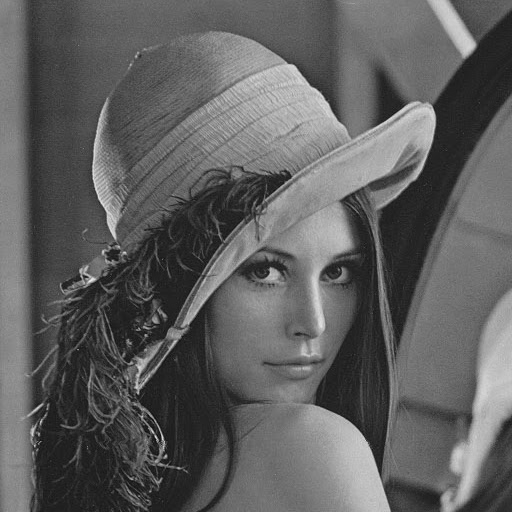
\includegraphics[width=4.5cm]{images/lenna.png} 
				\caption{Original image} 
				\label{subfig:org} 
			\end{subfigure} 
			~ 
			\begin{subfigure}{0.3\textwidth} 
				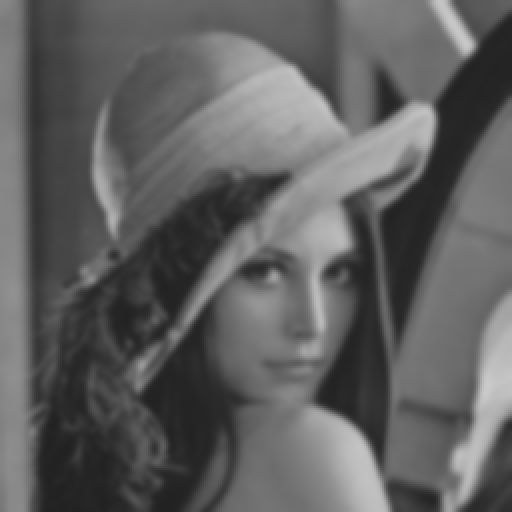
\includegraphics[width=4.5cm]{images/gaussian_at_sigma_3.png} 
				\caption{Gaussian with $\sigma = 3.2$} 
				\label{subfig:gauss1} 
			\end{subfigure} 
			~ 
			\begin{subfigure}{0.3\textwidth} 
				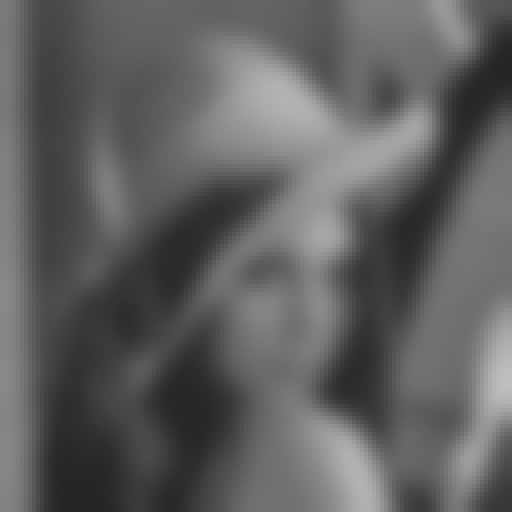
\includegraphics[width=4.5cm]{images/gaussian_at_sigma_10.png} 
				\caption{Gaussian with $\sigma = 10.?$} 
				\label{subfig:gauss2} 
			\end{subfigure} 
		
			\vspace{0.3cm} 
			
			\begin{subfigure}{0.3\textwidth} 
				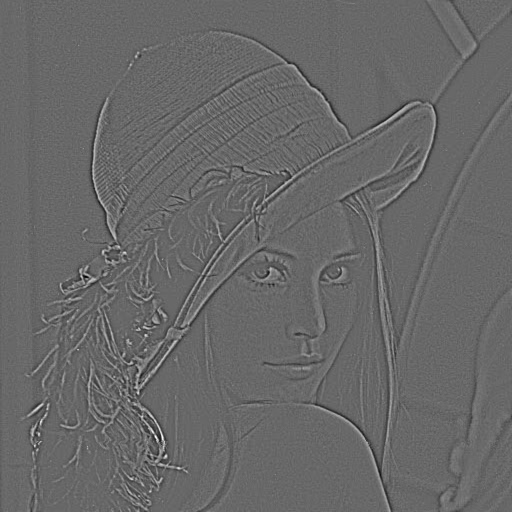
\includegraphics[width=4.5cm]{images/DoG_at_sigma_2.png} 
				\caption{DoG with $\sigma_1$=1.6?, $\sigma_2$=2.0?} 
				\label{subfig:org} 
			\end{subfigure} 
			~ 
			\begin{subfigure}{0.3\textwidth} 
				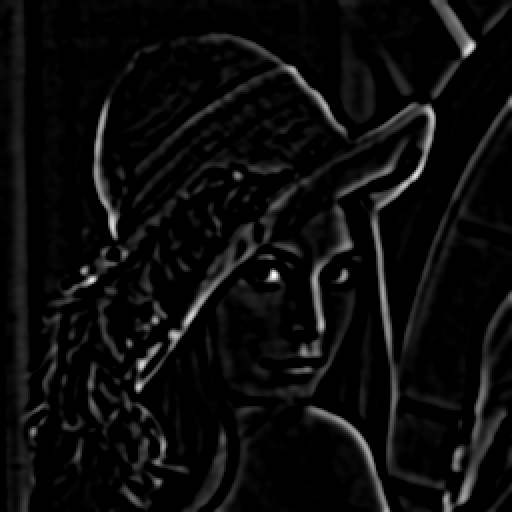
\includegraphics[width=4.5cm]{images/DoG_at_sigma_5.png} 
				\caption{DoG with $\sigma_1$=4?, $\sigma_2$=6?} 
				\label{subfig:org} 
			\end{subfigure} 
			~ 
			\begin{subfigure}[normla]{0.3\textwidth}  
				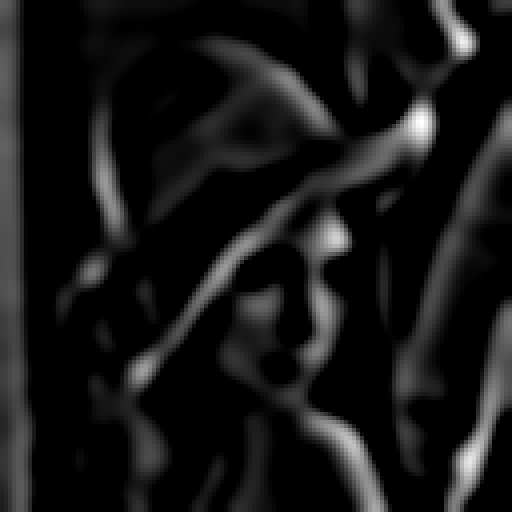
\includegraphics[width=4.5cm]{images/DoG_at_sigma_13.png} 
				\caption{DoG with $\sigma_1$=12?, $\sigma_2$=14?} 
				\label{subfig:org} 
			\end{subfigure} 
			\caption{This figure shows the impact of the Gaussian blur with different scales $\sigma$ on an image in its top row. Every image at the bottom depicts a normalized version of the difference between such two Gaussian images. A gray pixel value indicates no difference between the two Gaussians at that location, whereas black and white pixels reveal their disparity.  
				[original image taken from https://upload.wikimedia.org/wikipedia/en/2/24/Lenna.png]} 
		\end{center} 
	\end{figure} 

	In order to select keypoints from an image, Lowe uses a so-called scale-space representation of that image. To construct this scale-space, we first have to create multiple smoothed variations of our original image. We can smooth an image by convolving it with a 2D-Gaussian function $G(x, y, \sigma)$, where x and y are convolution directions and $\sigma$ is the standard deviation:
	
	$$
	G(x, y, \sigma) = \frac{1}{2 \pi \sigma^2} e^{-(x^2+y^2)/2\sigma^2}	
	$$
	
	The Gaussian blur is a low-pass filter that will suppress high frequencies which correspond to fine structures in the input image. The strenth of the blur is given by the standard deviation $\sigma$. The results of the Gaussian blurring can be seen in the top row of Figure 1. The resulting images stack-up to form a so-called Gaussian pyramid. 
	
	Lowe has found that using an initial scale $\sigma = 1.6$ and gradually adjusting each following scale of the Gaussian blur by a constant factor of $k = 2^{1/3}$ will achieve the best results [reference paper]. 
	
	After every three blurred images - which also means after each doubling of the $\sigma$ scale - the image can be down-sampled by a factor of two. All images of the same size in the pyramid are called an octave. The accuracy of sampling relative to $\sigma$ stays roughly the same for all octaves, but down-sampling the image results in major computational performance boosts. 
	
	If we take the difference between two Gaussian functions at different scales and convolve it with the original image, $I(x, y)$, we obtain the scale-space function $D(x, y, \sigma)$:
	
	\begin{eqnarray}
	D(x, y, \sigma) &=& (G(x, y, k\sigma) - G(x, y, \sigma)) \ast I(x, y) \\
	&=& (G(x, y, k\sigma) \ast I(x, y)) - (G(x, y, \sigma) \ast I(x, y))
	\end{eqnarray}

	
	The $\ast$ symbol is the convolution operator and due to its distributivity, we can also just subtract one Gaussian-blurred image pixelwise from another (2). The new image is called Difference of Gaussians (DOG). Doing this for every two neighboring images of the same octave in the Gaussian pyramid forms another pyramid of multiple Difference of Gaussians with one image less in each octave then before. In order to compensate for this lost image, we previously need to compute one more Gaussian blurred image at the end of each octave.
	
	
	%Keep in mind that the resampling for the first image of the next octave should to be done on the same image as before. 
	
	To finally retrieve the keypoints for our original image, each pixel of every Difference of Gaussian is compared to its eight pixel neighbors as well as its 18 neighbors from the DoGs lying directly above and below it in the pyramid (see Figure 2(b)). A pixel's location is taken into the set of our potential keypoints only if its value is either a minimum or a maximum in its surrounding neighborhood. Searching for extrema cannot be done on the first and last DoG image in each octave, since they only have one adjacent DoG of the same size, so they are omitted. Again, we need to generate two more Gaussians at the end of each octave, because it is favourable to extract extrema on three different sizes of $\sigma$ before moving on to the next octave. 
	
	As mentioned before, smoothing an image with different strengths results in images with different amount of detail. This is exactly what we need in order to find distinctive features no matter how large or small they are depicted in the picture. A minimum or maximum in scale-space means that a structure is still visible in one Gaussian image, but has been "smoothed away" by the stronger Gaussian kernel of the next. This leads to a large pixel value difference along the structure between these two Gaussians. A Difference of Gaussians has therefore a strong response to edges, as explicated in "Gaussian-based edge-detection methods-a survey" by M. Basu[reference]. 
	
	If we look at two images depicting the same object, but one taken from further away, we will still find corresponding keypoints, but on different scales in the DoG pyramid. This emphasizes the scale invariance property of SIFT features. 
	
	\begin{figure}[h]
		\begin{center} 
			\begin{subfigure}{0.5\textwidth} 
				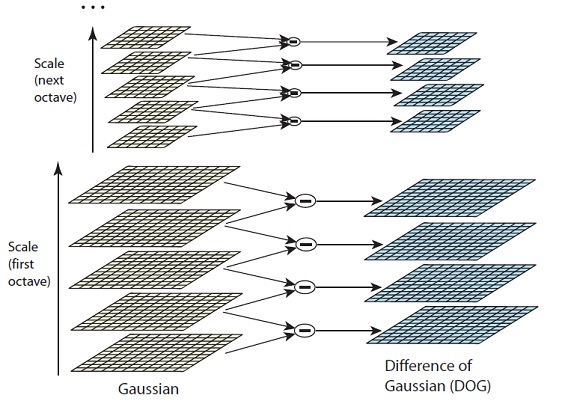
\includegraphics[width=7.5cm]{images/DoG_concept.jpg} 
				\caption{Constructing the Gaussian and Difference of Gaussian pyramid}
				\label{subfig:DoG_concept} 
			\end{subfigure} 
			~ 
			\begin{subfigure}{0.45\textwidth} 
				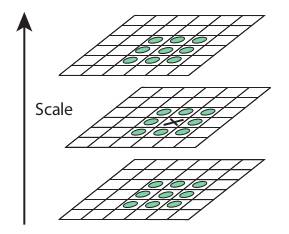
\includegraphics[width=6cm]{images/scale_space_extrema.jpg} 
				\caption{Finding scale-space extrema}
				\label{subfig:scale_space_extrema} 
			\end{subfigure} 
			 
			\caption{This figure shows the basic concept of finding scale-space extrema. Gaussian-blurred images with increasing standard deviation (from bottom to top) are depicted on the left side of (a). They are grouped by size, where each group forms an octave. Subtracting every two neighboured Gaussians results in a Difference of Gaussian (DoG) pyramid, shown in (a) on the right. 
			In (b) an "X"-marked pixel in one of these DoGs in being compared to its 26 neighbours, including those lying in adjacent DoGs. Only if that pixel holds the highest or lowest value of its surroundings it is considered to be a scale-space maximum or minimum, respectively.} 
		\end{center} 
	\end{figure} 
	
	
	\subsection{Keypoint refinement} 
	
	Our next step in the SIFT algorithm is to predict the precise location and scale of our previously extracted scale-space extrema. As an illustration example every image in DoG pyramid can also be represented as a 3D surface with pixel intensity values determining the expansion in the "z"-direction and interpolated values in between pixels as shown in Figure 3. We can improve our keypoints on a sub-pixel precision level by determining the exact locations of the peaks DoG surfaces.
	
	Let $\vec{x} = (x, y, \sigma)^T$ be the location and scale of a keypoint that we obtained in the previous section. For every such keypoint, we calculate a Taylor series expansion up to the quadratic terms of the scale-space function, $D(x, y \sigma)$, shifted by $\vec{x}$, so that the origin is at the keypoint's position.
	
	$$
	D(\vec{x}) = D + \frac{\partial D^T}{\partial\vec{x}} \vec{x} + \frac{1}{2}\vec{x}^T \\
	\frac{\partial^2D}{\partial\vec{x}^2}\vec{x}
	$$
	
	By calculating its derivative and setting it to zero, we receive another vector $\vec{o}$, which consist of the location and scale offset to our initial keypoint position $\vec{x}$.
	 
	\subsection{Keypoint filtering} 
	
	Some of the keypoints we obtained earlier might not be suitable for feature extraction due to a lack of contrast or unstable localization along an edge, so we need to reject such keypoints.
	  
	A low contrast also means that we might not find corresponding features in an image that has slightly been modified from the original. Contrast can easily be measured by the Taylor expansion of the scale space function shifted by the precise location $\hat x$ of the extremum: 
	
	$$ 
	D(\hat x) = D + \frac{1} {2} \frac{\partial D^T} {\partial x} \hat x 
	$$ 
	
	Lowe found that if the absolute value of that function is less than 0.03, then there is not enough contrast for a stable feature to be computed at that location. %(normalized pixel values [0..1]) 
	
	Even if a keypoint shows enough contrast, the algorithm might still struggle to accurately localize it along an edge. This is why we rather have corner-like keypoints than only edge-like. 
	
	To further illustrate this problem, we can simply look at an arbitrary thick white line on black background as shown in Figure 3(a). If we were to cut a patch from the middle section of the line (see Figure 3(b)), it would be impossible to tell at which exact location on the line the patch originated from. A patch of one of the end sections, as shown in 3(c), can easily be matched to its correct location at the corresponding end of the line. 
	
	In order to mathematically determine whether a given keypoint is corner-like and therefore stable or not, we can use a 2x2 Hessian matrix $H$, where $D_{xx}$, $D_{xy}$, $D_{yx}$ and $D_{yy}$ are approximated derivatives of the ..DoG.. using neighbouring sample points at the keypoints location and scale: 
	
	$$ 
	H = \begin{bmatrix} 
	D_{xx} & D_{xy} \\ 
	D_{yx} & D_{yy} \\ 
	\end{bmatrix} 
	$$ 
	
	Given $H$, we can look at the ratio of its two eigenvalues. If both eigenvalues are of the same magnitude, then we are dealing with a keypoint which shows a strong curvature. However, if one eigenvalue is significantly bigger than the other, we will discard this keypoint from our set, because it is unusable for our purposes due to its similarity to an edge. 
	
	
	\begin{figure}[h]
		\begin{center} 
			\begin{subfigure}{0.3\textwidth} 
				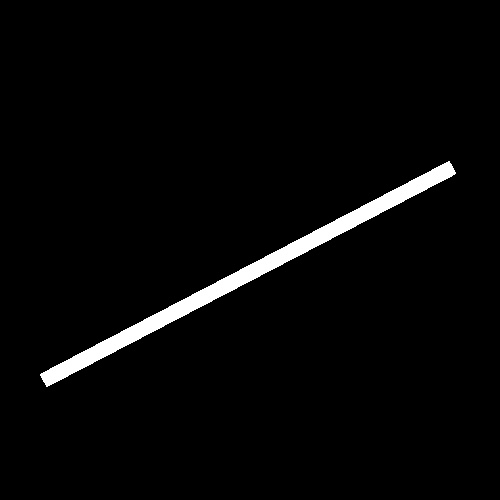
\includegraphics[width=4.5cm]{images/straight_line.png} 
				\caption{}
				\label{subfig:straigh_line} 
			\end{subfigure} 
			~ 
			\begin{subfigure}{0.3\textwidth} 
				
\includegraphics[width=4.5cm]{images/line_patch.png} 
				\caption{}
				\label{subfig:center_patch} 
			\end{subfigure} 
			~ 
			\begin{subfigure}{0.3\textwidth} 
				
\includegraphics[width=4.5cm]{images/corner_patch.png} 
				\caption{}
				\label{subfig:end_patch} 
			\end{subfigure}  
			\caption{The left image shows a straight line. The other two are up-scaled patches taken from the left image. Even for a human, it would be impossible to tell from which exact location the patch in the middle originally came from. However, the patch on the right can easily be localized at the left end of the line.} 
		\end{center} 
	\end{figure} 

	\subsection{Orientation assignment} 
	
	We have already shown that SIFT-Features are invariant to scale, but rotational invariance is just as important for numerus image processing tasks. For this purpose, Lowe assigns each keypoint one or more consistent orientations, based on its neighborhood's gradients. An image gradient indicates a change of pixel intensity in a specific direction.  
	
	The most prominent gradient direction of a keypoint seems to be a good pick for assignment of a consistent orientation, because rotating an image by an angle $\phi$ will only shift all gradients by $\phi$ as well; thus, maintaining the same relative directions. 
	
	To find the most prominent gradient direction, we first need to compute all gradients around a keypoint and organize them in a histogram. A histogram shows the distributing of numerical data by dividing the data in disjoint categories, called bins. In our application we will have 36 bins and each bin represents a range of 10� out of all 360� possible angle directions.  
	
	For every Gaussian blurred image, L, all gradient directions and magnitudes are precomputed for performance purposes. 
	The direction of a gradient at a certain location in L can be calculated with the following formula using pixel differences: 
	
	$$ 
	\theta(x, y) = \tan^{-1}{((L(x, y + 1) - L(x, y - 1)) / (L(x + 1, y) - L(x - 1, y)))} 
	$$ 
	
	The gradient's magnitude shows how strong the pixel intensity changes in the gradient's direction. It can be calculated in a similar manner: 
	
	$$ 
	m(x, y) = \sqrt{(L(x + 1, y) - L(x - 1, y))^2 + (L(x, y + 1) - L(x, y - 1))^2} 
	$$ 
	
	The magnitude of each gradient is weighted by a Gaussian function, so that gradients closer to the center of the keypoint have a higher impact than gradients further away which tend to be more unstable to minor transformations. This weighted input will be added to the bin which represents the gradient's direction. The highest peak in that histogram is the direction we are looking for. Any other peak that holds a value higher than 80\% of the highest peak leads to the creation of an additional keypoint at the same location, but with a different orientation. These keypoints with multiple strong gradient directions are scarce, but help to make matching significantly more stable.  
	
	A parabola is fit to the three closest values of each peak to achieve a more accurate orientation at the real maximum of that peak. 
	
	%(Picking up the patch matching problem of a straight line from earlier (Figure 3). Both end patches would generate similar descriptors after they have been assigned an orientation, thus matching their keyypoints could proof problematic) 
	
	\subsection{Constructing the feature descriptor} 
	
	There are many possibilities to describe the area around a keypoint. For instance we could be storing the intensity or color values inside our feature descriptor. However, the disadvantage of this approach is that many images are taken under different lighting conditions. Hence intensity values of corresponding keypoints might vary a lot. Image gradients are a better choice for constructing a feature descriptor, because they only coincide with change of pixel intensity, rather than intensity values itself.  
	
	%relative gradient directions / rotated 16x16 neighbourhood 
	
	SIFT uses all gradients within a 16x16 neighbourhood around each keypoint. These gradients will further be organized in 4x4 cells, so there will be a total of 16 cells. Analogous to section 2.4 each cell accumulates its gradients in an orientation histogram, but this time with only 8 bins. Hence each bin represents 45� which allows for small inaccuracies of the gradients directions, but keeps the final descriptor small.
	 
	The feature descriptor is actually just a sequence of linking all values of every cell histogram together in a consistent manner.  Every keypoint uses 4x4 cells with 8 orientation bins each. Thus accumulating all these values in a single descriptor, results in a 128 dimensional vector. 
	
	Experiments show that normalizing the vector to unit length helps to cope with illumination changes. By limiting every orientation value in the cell histogram to a maximum of 0.2, we guarantee that no single dominant gradient can suppress the other gradients. Have multiple strong orientations in our final descriptor is more desirable than having a single dominant one, because "non-linear illumination changes can also occur due to camera saturation or due to illumination changes that affect 3D surfaces with differing orientations by different amounts" [Zitat 6.1 paper]. 
	
	%\section{(Matching)} 
	
	\section{Problematic situations} 
	
	We have seen that SIFT features are highly thought-out, but of course they might fail their purpose in some situations. 
	SIFT features can be computed relatively fast, however matching over a vast database might still take a long time. Herbert Bay addresses this problem in his publication "Speeded Up Robust Features" (SURF) from 2006. His SURF features are based on SIFT and can be computed even faster. Their smaller 64 dimensional descriptor allows for faster matching of its features with only minor loss in accuracy. Hence they might be better suited for some applications which require real-time. 
	
	In one picture a subject might be well lit by sunshine, whereas another picture of the same scene might be taken in cloud weather. The first will have a strong contrast due to shadows, whereas the other will have flat contrast. As mentioned in the previous section, the large magnitude of strong gradients is being restrained and normalized when constructing the feature descriptor, so the deviation of contrast only shows a weak impact on the final feature descriptor. However, Shadows also tend to cause strong gradients in a direction which is determined, not by the object, but the position of the light source. This might lead to the corruption of some feature descriptors. 
	
	%problem with outliers, (RANSAC?)
		
	%When it comes to matching feature descriptors we will almost always choose some false correspondences. These outliers need to be excluded 
	
	Another difficult situtation might be if an picture shows multiple occurrences of the same thing. Having repetitive structures in one scene will most likely lead to false matches of correspondences, called outliers. For instance a fence consists of many pickets, so its feature descriptors might be fairly similar which only vary due to the diversity of the background. 
	
	%\begin{figure}[!hb]
	%	\begin{center} 
	%		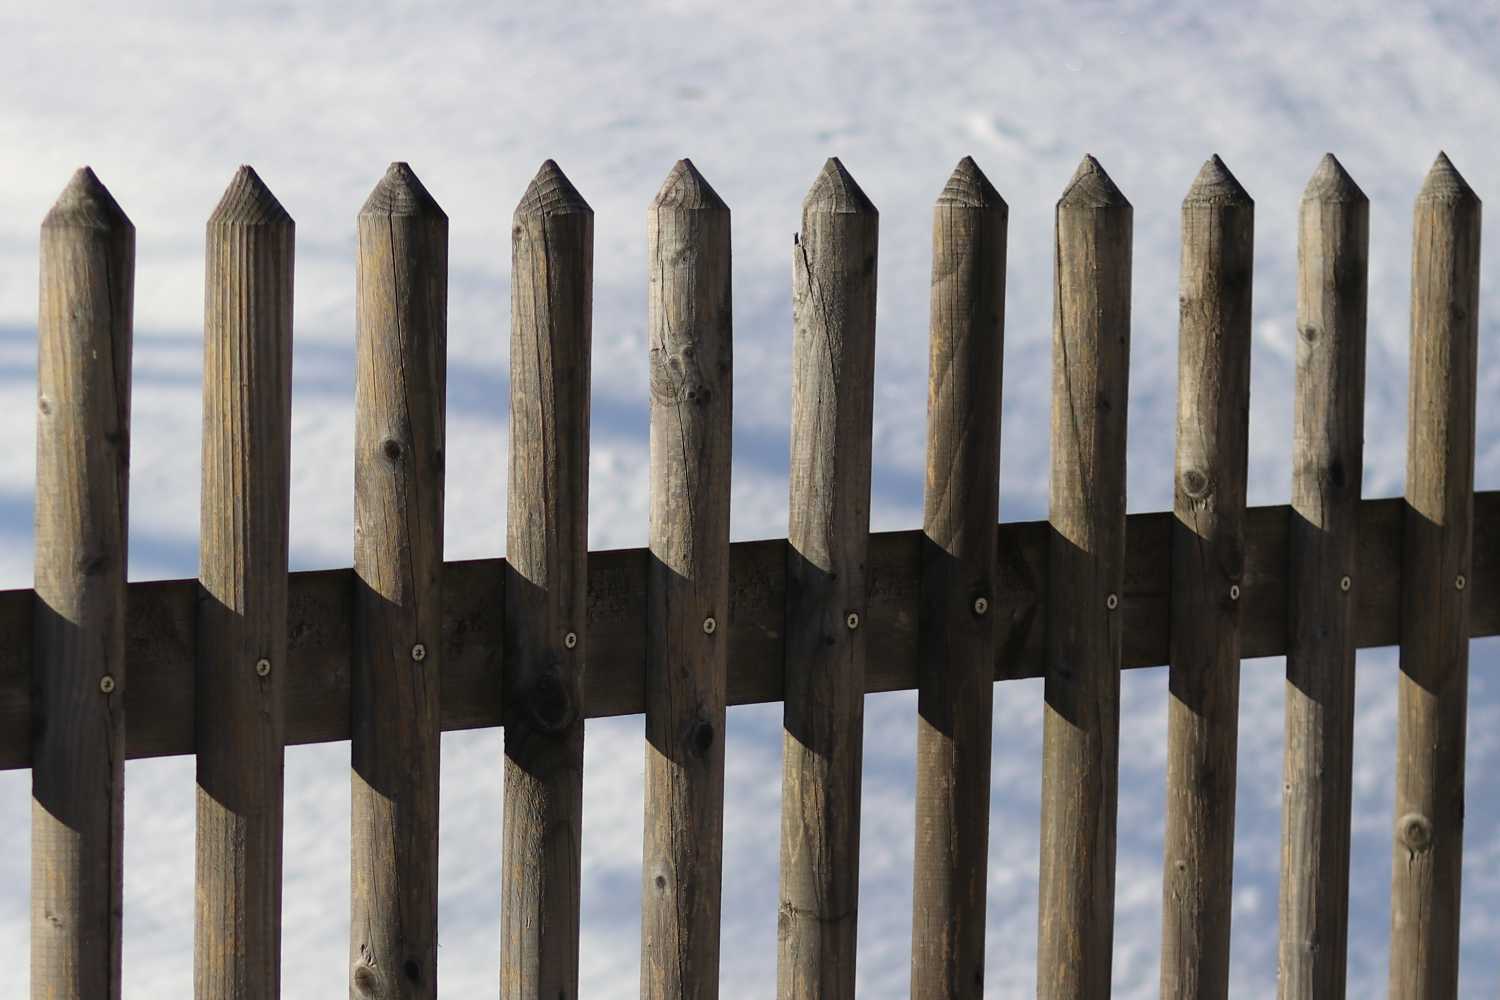
\includegraphics[width=12cm]{images/fence.png} 
	%		\label{subfig:fence} 
	%
	%		\caption{} 
	%	\end{center} 
	%\end{figure} 
	
	%An easy fix for this problem would be to only accept matches if the 
	
	%Outlier detection is essential 
	
	%Robustness only to a certain point 
	
	\section{Conclusion} 
	
	The SIFT algorithm is a great way to extract distinct points from an image and describe their surrounding area by constructing a feature descriptor in an invariant manner. These descriptors can in turn be used to match corresponding points across images. Their invariance and robustness properties allow for stable matching even if the reference images differ in scale, rotation or lighting of the depicted object(s).
	
	Slight changes in 3D viewing angle are also accounted for. Correctly matching a small amount of these distinct points is the major foundation of many image processing tasks like object recognition, panorama stitching and gesture recognition. 
	
	SIFT features are not perfect for every situations as shown in the last section. Nevertheless, the Scale Invariant Feature Transform has been a milestone in computer vision and provided the fundamentals for many following image feature-based algorithms. 
	
\end{document} 


